\documentclass[document.tex]{subfiles}

\begin{document}

\section{S1 - Introduction à l'espace d'état}

\begin{enumerate}
\item Variable d'état
\item Représentation d'un système LTI dans l'espace d'état
\item Exemple temps continue et temps discret
\item Systèmes LTI représentables dans l'espace d'état
\item Interconnexion de systèmes dans l'espace d'état
\item Conversion espace d'état $\rightarrow$ fonction de transfert
\item Pôles, valeurs propres de la matrice système A, stabilité
\end{enumerate}

\subsection{Nouveaux concepts}
La régulation avancée a besoin d'un certain nombre de concepts, tel que \textbf{l'espace d'état}.\\

Il s'agit d'une manière de représenter un système LTI.\\

Dans un premier temps, nous allons nous familiariser avec l'espace d'état \textbf{sans parler de régulation}.

\subsection{Introduction - l'espace d'état}

Représentations de systèmes \textbf{LTI} (linéaires et invariant dans le temps) :

\begin{center}
domaine \textbf{fréquentiel} :  \hfill domaine \textbf{temporel} : \\
fonction / matrice de transfert  		\hfill $\rightarrow$ \hfill équations différentielles
\end{center}

L'espace d'état (state space) est une représentation dans le domaine temporel
qui fait intervenir des variables que l'on appelle variables d'état $ x_k(t) $, $ k = 1 \ldots N $. \\
Chaque variable d'état est liée au : 
\begin{itemize}
\item stockage de matière, ou
\item stockage d'énergie, ou
\item stockage d'information (numérique)
\end{itemize}

\subsection{Variable d'état}
\begin{center}
\textbf{Les variables d'états sont tout les paramètres qui varie en fonction d'une référence (souvent en fonction du temps)}
Il faut donc trouver quelles paramètres \textbf{varie} :
\begin{enumerate}
\item \large Dérivée : $\boxed{f(t)= c \cdot \frac{d x}{d t}}$
\item \large Intégral : $\boxed{f(t) = \int_0^t x(\tau)d\tau}$
\end{enumerate}
\end{center}
\subsubsection{Exemple 1 - Stockage de matière}
\begin{figure}[H]
    \centering
    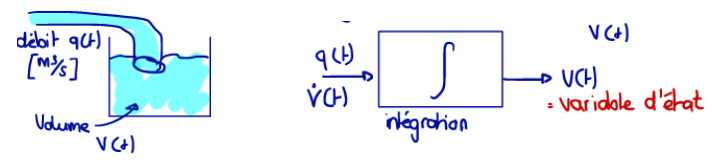
\includegraphics[width=0.8\textwidth]{Include/Figure/1.png}
\end{figure}
\begin{itemize}
\item la sortie d'un intégrateur correspond à une variable d'état
\item une variable d'état porte une dérivée
\item techniquement parlant, une variable d'état ne peut pas sauter
\item le signal de \textbf{sortie} d'un système \textbf{peut} correspondre à une variable d'état
\item le signal d'\textbf{entrée} n'est \textbf{jamais} une variable d'état
\end{itemize}

\subsubsection{Exemple 2 - Électricité}

Capacité :
\begin{equation}
	i_c(t) = C \cdot \frac{dU_c}{dt}
\end{equation}
\begin{figure}[H]
    \centering
    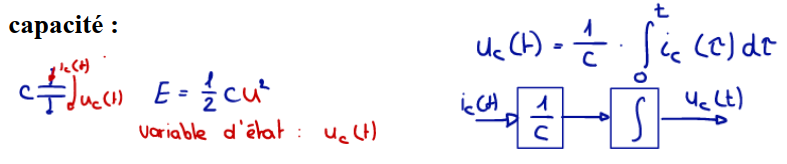
\includegraphics[width=0.8\textwidth]{Include/Figure/4.png}
\end{figure}

Inductance :
\begin{equation}
	U_L(t) = L \cdot \frac{di_L}{dt}
\end{equation}
\begin{figure}[H]
    \centering
    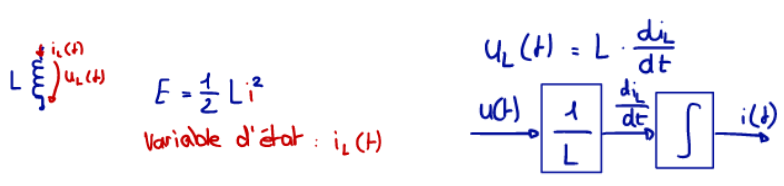
\includegraphics[width=0.8\textwidth]{Include/Figure/5.png}
\end{figure}

\subsubsection{Exemple 3 - Mécanique}

Énergie potentielle : \hfill Avec $\Delta L$ : déplacement $[m]$
\begin{equation}
 	E_{pot}=\frac{1}{2}k \cdot \Delta L^2 
\end{equation}
\begin{figure}[H]
    \centering
    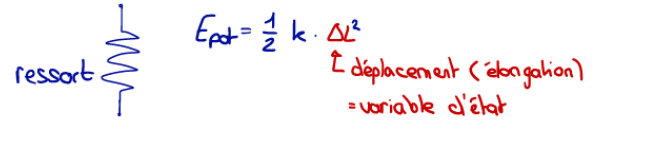
\includegraphics[width=0.8\textwidth]{Include/Figure/6.png}
\end{figure}

Énergie cinétique :	\hfill Avec $v$ : vitesse $[\frac{m}{s}]$
\begin{equation}
	E_{cin}=\frac{1}{2}m \cdot v^2
\end{equation}
\begin{figure}[H]
    \centering
    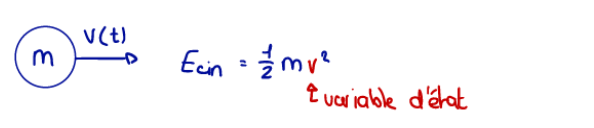
\includegraphics[width=0.8\textwidth]{Include/Figure/7.png}
\end{figure}

Chaque degré de liberté (DDL) mécanique fait intervenir deux variables
d'état :
\begin{enumerate}
\item \textbf{position}
\item \textbf{vitesse}
\end{enumerate}

\subsection{Espace d'état}

\textbf{Moyen mnémotechnique : } Espace d'état $\rightarrow$ \textbf{SYS-EN-SOR-BY} (\textit{600 sorbet})\\[6pt]

\begin{itemize}
	\item A : Matrice de \textbf{système} $n\times p$
	\item B : Matrice d'\textbf{entrée} $n\times p$
	\item C : Matrice de \textbf{sortie} $r\times n$
	\item D : Matrice de \textbf{bypass} $r\times p$
\end{itemize}


\subsection{Vecteur d'état}
Toutes les variables d'état sont regroupées dans le vecteur d'état

\subsubsection{Continue}
\begin{equation}
	\vec{x}(t) = \begin{bmatrix}
		x_1(t) \\ x_2(t) \\ \vdots \\ x_m(t)
	\end{bmatrix} \rightarrow m : ordre \; du \; système
\end{equation}

La représentation dans l'espace d'état d'un système correspond à un système d'équations différentielles, chacune de degré 1.\\

Elle peut être décrite avec l'aide de 4 matrices A, B, C, D :

\begin{equation}
\boxed{
\begin{array}{r c l}
		\dot{x} & = & Ax + Bu \\
		y       & = & Cx + Du
\end{array}
}
\end{equation}

\subsubsection{Discret}
\begin{equation}
	\vec{x}[k] = \begin{bmatrix}
		x_1[k] \\ x_2[k] \\ \vdots \\ x_n[k]
	\end{bmatrix} \rightarrow n : ordre \; du \; système
\end{equation}

Elle peut être décrite avec l'aide de 4 matrices A, B, C, D :

\begin{equation}
\boxed{
\begin{array}{r c l}
		x[k+1] & = & A_nx[k] + B_nu[k] \\
		y[k]   & = & Cnx[k] + D_nu[k]
\end{array}
}
\end{equation}

\begin{equation}
\begin{array}{l c c c r}
	\frac{1}{s} & = & intégrer & \rightarrow & \frac{1}{z} = retarder \\
	s & = & dériver & \rightarrow & z = avancer
\end{array}
\end{equation}

\begin{figure}[H]
	\centering
	\begin{subfigure}[b]{0.64\textwidth}
		\centering
		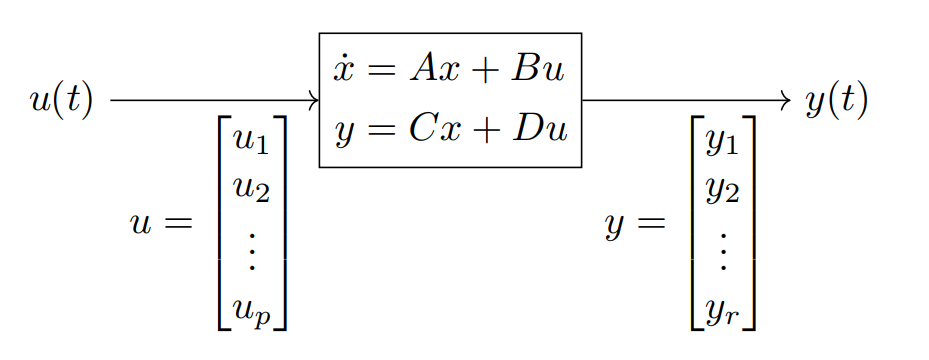
\includegraphics[width=\textwidth]{Include/Figure/8.png}
	\end{subfigure}
	\hfill
	\begin{subfigure}[b]{0.34\textwidth}
		\centering
		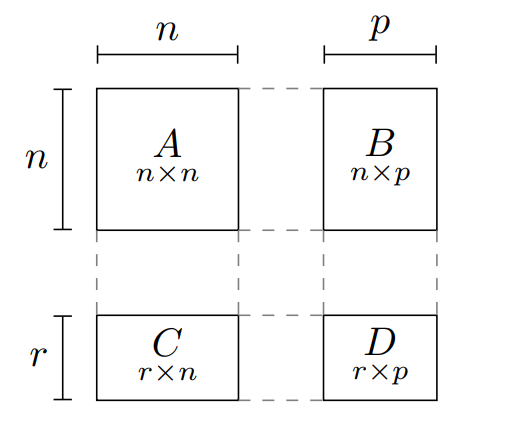
\includegraphics[width=\textwidth]{Include/Figure/9.png}
	\end{subfigure}
\end{figure}

\subsection{Lien avec un schéma bloc}
\begin{figure}[H]
    \centering
    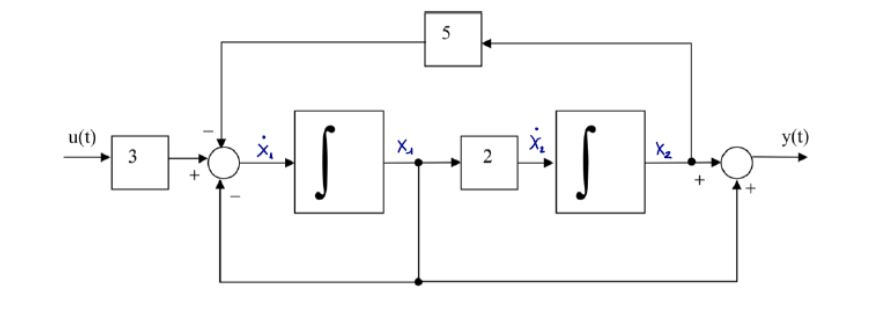
\includegraphics[width=0.9\textwidth]{Include/Figure/12.png}
\end{figure}

A partir d'un schéma bloc, on peut directement lire les matrices A, B, C et D.
La numérotation des variables d'état est libre.
\begin{center}
	$ A = \begin{bmatrix} -1 & -5 \\ 3 & 0 \end{bmatrix} $ \hfill
	$ B = \begin{bmatrix} 3 \\ 0 \end{bmatrix} $ \hfill
	$ C = \begin{bmatrix} 1 & 1 \end{bmatrix} $ \hfill
	$ D = \begin{bmatrix} 0 \end{bmatrix} $
\end{center}

\textbf{Bloc de base : }
\begin{enumerate}
\item intégrateur
\item gains
\item sommateur / soustracteur
\end{enumerate}

\begin{center}
\textbf{Lois de physique de base} (Kirchoff, Newton,...) \\
$ \updownarrow $ \\
\textbf{Schéma bloc} \\
$ \updownarrow $ \\
\textbf{Représentation dans l'espace d'état} (matrice A, B, C, D)
\end{center}

Système analogique (Matlab): 
\begin{itemize}
\item Domaine fréquentiel : G = tf(num,den), tf = transfert function
\item Domaine temporel :  G = ss(A,B,C,D), ss = state space
\end{itemize}

\subsection{Exemple : Espace d'état numérique}

\begin{figure}[H]
    \centering
    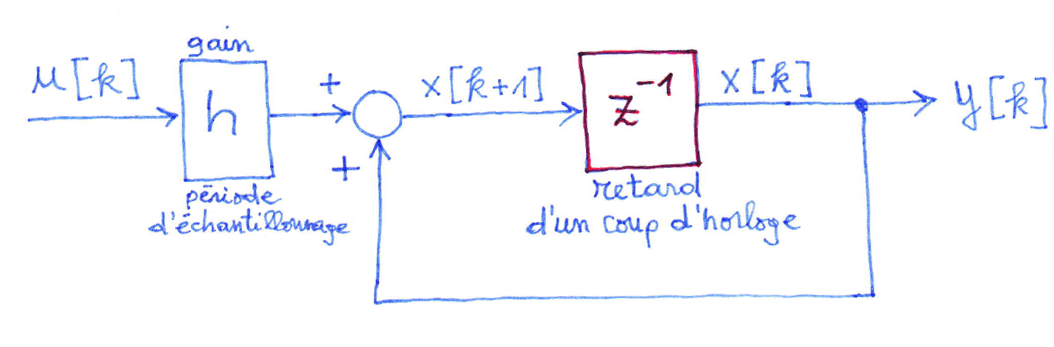
\includegraphics[width=0.9\textwidth]{Include/Figure/17.png}
\end{figure}

\textbf{A quoi correspond ce système ?}
Intégrateur numérique avec la méthode des rectangles !\\

\begin{equation}
\begin{array}{c c c}
	A_n = 1 & \; & B_n = h \\
	C_n = 1 & \; & D_n = 0
\end{array}
\end{equation}

\subsubsection{Règle de Mason}

\begin{itemize}
\item Regarder la contre réaction
\item Regarder la polarité de la somme de la contre réaction
\end{itemize}
\begin{equation}
	\boxed{G(z) = K \cdot \frac{A}{1 -(pol_{sum})A} = \frac{h \cdot z^{-1}}{1-z^{-1}} = \frac{h}{z-1}}
\end{equation}

\subsubsection{Schéma bloc « vectoriel » associé}

\textbf{Temps continue}

\begin{figure}[H]
    \centering
    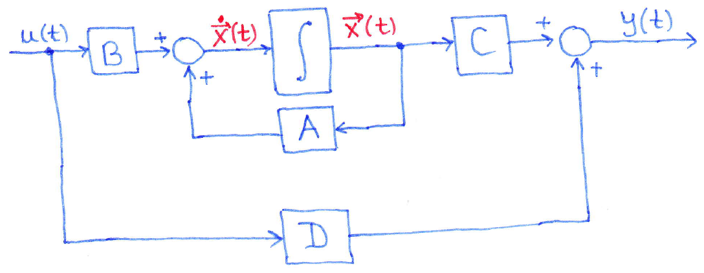
\includegraphics[width=0.7\textwidth]{Include/Figure/15.png}
\end{figure}

\textbf{Temps discret}

\begin{figure}[H]
    \centering
    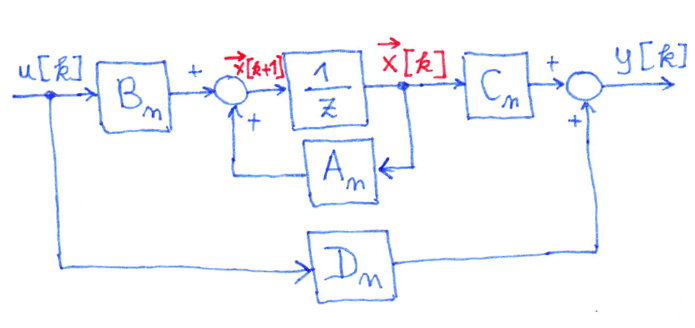
\includegraphics[width=0.7\textwidth]{Include/Figure/16.png}
\end{figure}

\subsection{Exemple de modélisation dans l'espace d'état}

\begin{figure}[H]
    \centering
    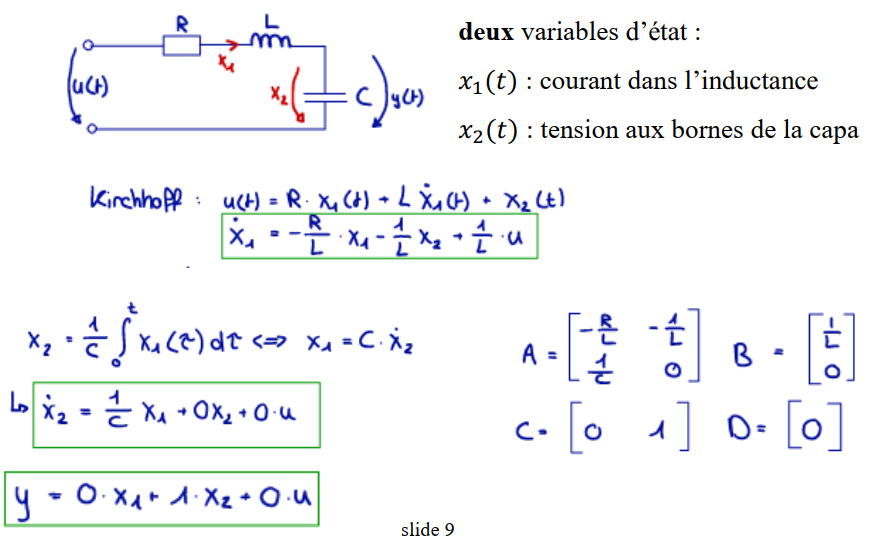
\includegraphics[width=0.9\textwidth]{Include/Figure/11.png}
\end{figure}

\subsection{Exemple : système mécanique à 2 DDL (2 degrés de libertés)}

\begin{figure}[H]
    \centering
    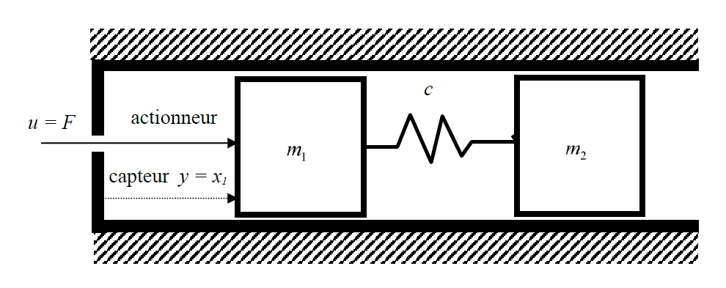
\includegraphics[width=0.9\textwidth]{Include/Figure/18.png}
\end{figure}

Deux degrés de libertés (DDL) $\rightarrow$ 4 variables d'états
\begin{equation}
	x = \begin{bmatrix}
		x_1 \\ x_2 \\ v_1 \\ v_2
	\end{bmatrix} = \begin{bmatrix}
	x_1 \\ x_2 \\ x_3 \\ x_4
	\end{bmatrix}
\end{equation}

\begin{figure}[H]
    \centering
    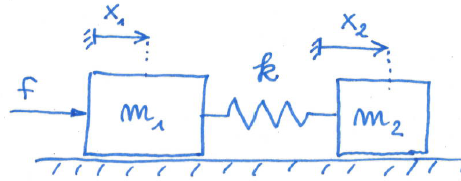
\includegraphics[width=0.6\textwidth]{Include/Figure/19.png}
\end{figure}

Loi de Newton pour chaque masse (isoler les corps !)\\

\begin{equation}
\begin{cases}
	m_1 \ddot{x_1} = f-k(x_1-x_2) \\
	m_2 \ddot{x_2} = k(x_1-x_2)
\end{cases}
\end{equation}

If faut d'abord trouver les relations qui décrivent l'espace d'état en isolant chaque dérivé de $x$ :
\begin{equation}
\begin{array}{c}
	\dot{x_1} = v_1 = x_3 \\[12pt]
	\dot{x_2} = v_2 = x_4 \\[12pt]
	\dot{x_3} = \dot{v_1} = \ddot{x_1} = -\frac{k}{m_1}x_1 + \frac{k}{m_1}x_2 + \frac{1}{m_1}f \\[12pt]
	\dot{x_4} = \ddot{x_2} =\frac{k}{m_2}x_1 - \frac{k}{m_2}x_2;
\end{array}
\end{equation}
\\[12pt]
\begin{equation}
\begin{array}{c c}
	A = \begin{bmatrix}
	0 & 0 & 1 & 0 \\ 0 & 0 & 0 & 1 \\ -\frac{k}{m_1} & \frac{k}{m_1} & 0 & 0  \\ \frac{k}{m_2} & -\frac{k}{m_2} & 0 & 0
	\end{bmatrix} & B = \begin{bmatrix}
	0 \\ 0 \\ \frac{1}{m_1} \\ 0
	\end{bmatrix} \\
	\; & \; \\
	C = \begin{bmatrix}
	1 & 0 & 0 & 0
	\end{bmatrix} & D = 0
\end{array}
\end{equation}

Si on s'intéresse au déplacement \textbf{des deux masses}, la \textbf{matrice de sortie $C$} devient:
\begin{equation}
	C = \begin{bmatrix}
		1 & 0 & 0 & 0 \\
		0 & 1 & 0 & 0
	\end{bmatrix}
\end{equation}

\subsection{Exemple "Balle de golf"}

\begin{figure}[H]
    \centering
    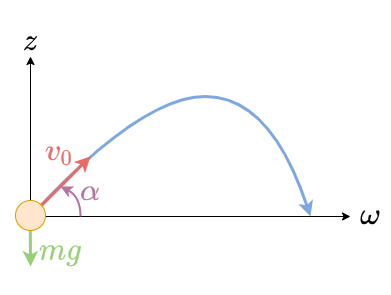
\includegraphics[width=0.5\textwidth]{Include/Figure/30.png}
\end{figure}


Hypothèse : pas de frottement de l'aire\\
Newton :
\begin{equation}
z = \frac{1}{m}\big(\sum F\big)
\end{equation}

On constate qu'il y a \textbf{deux degré de liberté}, il faut donc \textbf{quatre variables d'états}

\begin{equation}
 \vec{x} = \begin{bmatrix}
 	\omega \\ z \\ v_\omega \\ v_z
 \end{bmatrix} = \begin{bmatrix}
 	x_1 \\ x_2 \\ x_3 \\ x_4
 \end{bmatrix}
\end{equation}

Nous pouvons directement trouver le vecteur initiale : \\

\begin{equation}
 \vec{x}_0 = \vec{x}(0) = \begin{bmatrix}
 	0 \\ 0 \\ v_0 \cdot cos(\alpha) \\ v_0 \cdot sin(\alpha)
 \end{bmatrix}
\end{equation}

If faut d'abord trouver les relations qui décrivent l'espace d'état en isolant chaque dérivé de $x$ :
\begin{equation}
\begin{array}{c}
	\dot{x_1} = \dot{\omega} = v_{\omega} = x_3 \\[12pt]
	\dot{x_2} = \dot{z} = v_z = x_4 \\[12pt]
	\dot{x_3} = \dot{v}_{\omega} = acc_{horizontal} = 0 \; : \; \text{(mvt MRU)} \\[12pt]
	\dot{x_4} = \dot{v}_{z} = acc_{vertical} = -g
\end{array}
\end{equation}
\\[12pt]
\begin{equation}
\begin{array}{c c}
	A = \begin{bmatrix}
	0 & 0 & 1 & 0 \\ 0 & 0 & 0 & 1 \\ 0 & 0 & 0 & 0 \\ 0 & 0 & 0 & 0
	\end{bmatrix} & B = \begin{bmatrix}
	0 \\ 0 \\ 0 \\ -1
	\end{bmatrix} \\
	\; & \; \\
	C = \begin{bmatrix}
	1 & 0 & 0 & 0 \\
	0 & 1 & 0 & 0
	\end{bmatrix} & D = \begin{bmatrix}
	0 \\ 0
	\end{bmatrix}
\end{array}
\end{equation}




\subsection{Taille des matrice A, B, C et D}

\begin{figure}[H]
    \centering
    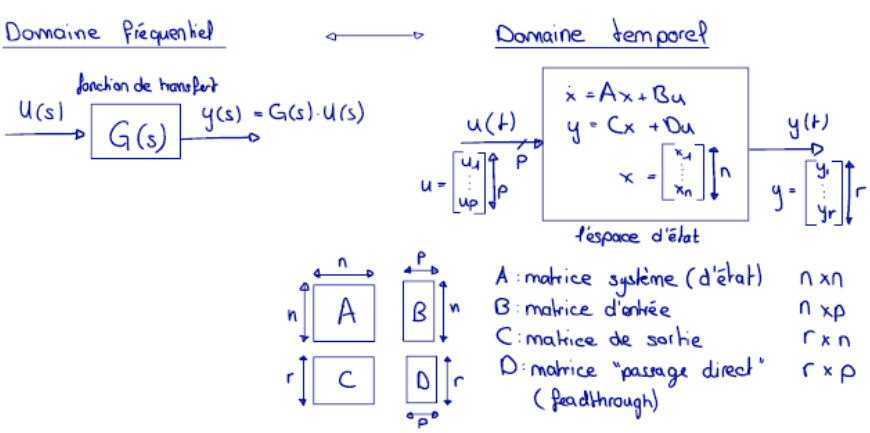
\includegraphics[width=\textwidth]{Include/Figure/13.png}
\end{figure}

\subsection{schéma bloc "vectoriel" associé}

\begin{figure}[H]
    \centering
    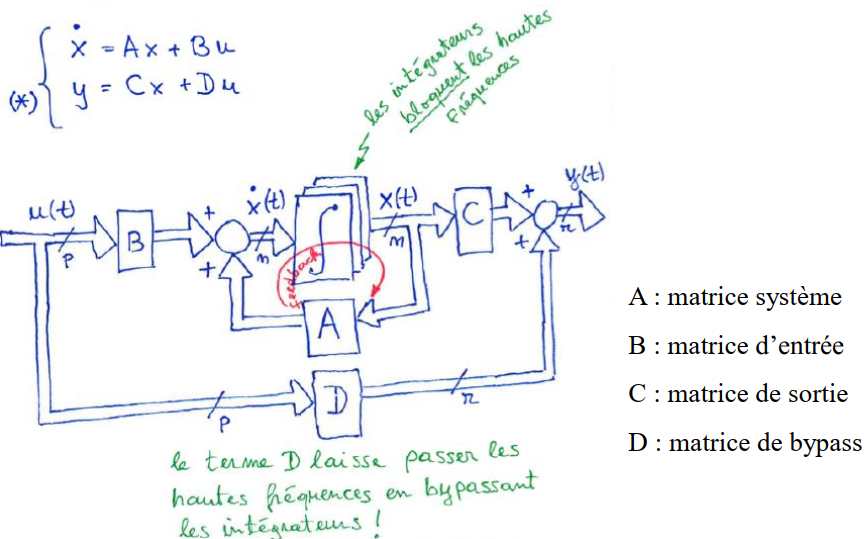
\includegraphics[width=\textwidth]{Include/Figure/14.png}
\end{figure}


\subsection{Exemple Modélisation d'un moteur DC dans l'espace d'état}
\begin{figure}[H]
    \centering
    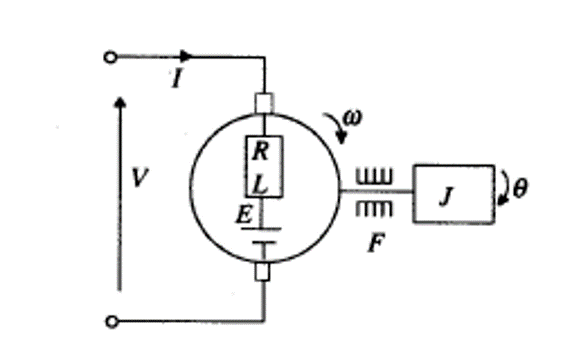
\includegraphics[width=0.5\textwidth]{Include/Figure/20.png}
\end{figure}
\begin{itemize}
\item Signal d'entrée : tension u(t)
\item Signal de sortie : position angulaire $\theta(t)$
\end{itemize}
Choix du vecteur d'état :
\begin{equation}
	x = \begin{bmatrix}
	 x_1 \\ x_2 \\ x_3
	\end{bmatrix} = \begin{bmatrix}
	\theta \\ \omega \\ i
	\end{bmatrix} = \begin{bmatrix}
	\text{Position angulaire} \\ \text{Vitesse angulaire} \\ \text{Courant dans le bobinage}
	\end{bmatrix}
\end{equation}

\subsubsection{Modélisation dans l'espace d'état}

\begin{tabular}{l l}

Couple entraînant : & $T_{entr}(t)=K_t \cdot i(t)$ \\
Tension induite : & $ u_i(t) = K_e \cdot
\omega(t) $ \\
Newton : & $ J\dot{\omega} = -R_f\omega+T_{entr} \Rightarrow \dot{x}_2=\frac{R_f}{J}x_2 + \frac{K_t}{J}x_3$\\
Kirchoff : & $u = Ri+L\frac{di}{dt}+u_i \Rightarrow \dot{x}_3 + \frac{1}{L}u$ 
\end{tabular}
\\[12pt]
Ce qui donne l'espace d'état : 

\begin{equation}
\begin{array}{c c c c}
	A = \begin{bmatrix}
		0 & 1 & 0 \\ = & -\frac{R_f}{J} & \frac{K_t}{J} \\ 0 & -\frac{K_e}{L} & -\frac{R}{L}
	\end{bmatrix} & B = \begin{bmatrix}
	0 \\ 0 \\ \frac{1}{L}
	\end{bmatrix} & C = \begin{bmatrix}
	1 & 0 & 0 
	\end{bmatrix} & D = 0
\end{array}
\end{equation}

\subsection{Avantage de la représentation dans l'espace d'état}

\begin{itemize}
	\item Permet de simuler le comportement à partir de conditions initiales non nulles
	\item Contrairement à la fonction de transfert, qui est une représentation I/O, la représentation dans l'espace fait apparaître des grandeurs internes, les variables d'état, ayant une signification physique utile
	\item La représentation dans l'espace d'état est de nature vectorielle/matricielle, bien adapté aux calculs sur ordinateur
\end{itemize}


\subsection{Système LTI représentables dans l'espace d'état}
\textbf{Quels systèmes LTI ne sont pas représentables dans l'espace d'état ?} \\
Systèmes à comportement \textbf{dérivateur}, resp. systèmes ayant une fonction de transfert à \textbf{degré relatif négatif} (gain haute fréquence infini).\\
On peut remédier en introduisant une matrice \textbf{E} \textbf{non inversible} à gauche.\\

système "descripteur" utilisé plutôt rarement, sauf pour calculer l'inverse d'un système.

\begin{equation}
\begin{cases}
	E \dot{x} = Ax + Bu \\
	y = Cx + Du \\
\end{cases}
\end{equation}

Exemple : \\
\begin{center}
$
\begin{array}{l}
	\begin{bmatrix}
		0 & 0 \\ 0 & 0 \end{bmatrix} \begin{bmatrix}
		\dot{x_1} \\ \dot{x_2}
		\end{bmatrix} = \begin{bmatrix}
		1 & 0 \\ 0 & 1
		\end{bmatrix} \begin{bmatrix}
		x_1 \\ x_2
		\end{bmatrix} + \begin{bmatrix}
			0 \\ -1
		\end{bmatrix} u \\[24pt]
		y = \begin{bmatrix}
		1 & 0 \end{bmatrix} \begin{bmatrix}
		x_1 \\ x_2 \end{bmatrix} + 0 \cdot u \\[24pt]
		\text{Dérivateur : } y \; = \; \dot{u}
\end{array}
$
\end{center}


\subsection{Interconnecter de plusieurs systèmes dans l'espace d'état}

\subsubsection{Mise en cascade}
\begin{figure}[H]
    \centering
    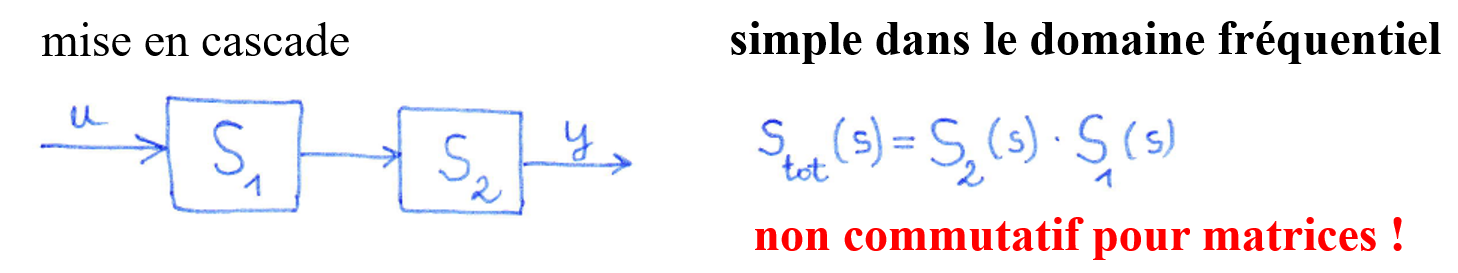
\includegraphics[width=0.8\textwidth]{Include/Figure/21.png}
\end{figure}

\subsubsection{Mise en parallèle}
\begin{figure}[H]
    \centering
    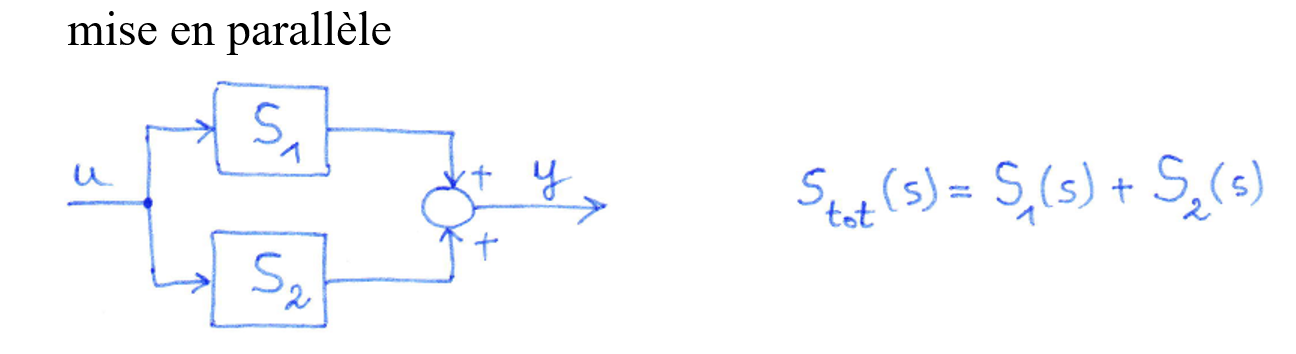
\includegraphics[width=0.8\textwidth]{Include/Figure/22.png}
\end{figure}

\subsubsection{Mise en contre-réaction}
\begin{figure}[H]
    \centering
    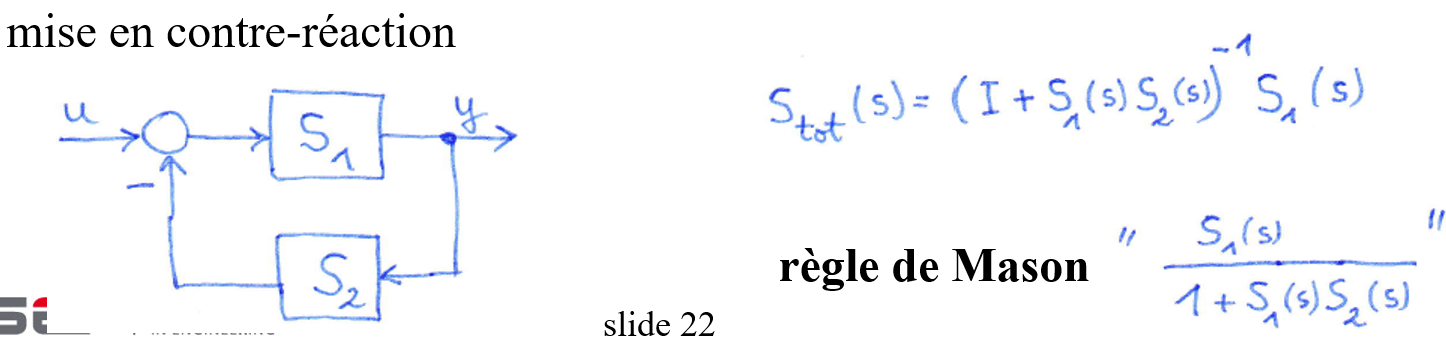
\includegraphics[width=0.8\textwidth]{Include/Figure/23.png}
\end{figure}

\subsubsection{Concaténation des vecteurs d'état des sous systèmes}

\begin{itemize}
 \item Chaque sous-système a son propre vecteur d'état qui "vit dedans".
 \item Le vecteur d'état global est la concaténation de ces N sous-vecteurs.
 \item Les matrices d'état global se calculent en prenant en compte les équations des N sous-systèmes et les équations liées à leurs interconnexions.
\end{itemize}

\begin{figure}[H]
    \centering
    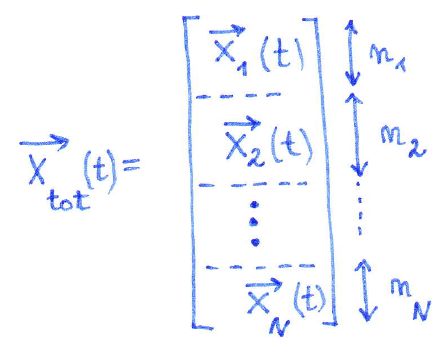
\includegraphics[width=0.4\textwidth]{Include/Figure/24.png}
\end{figure}

\subsubsection{Exemple : mise en parallèle}

\begin{figure}[H]
    \centering
    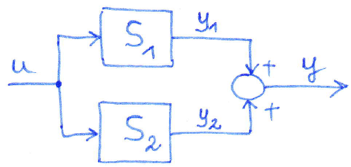
\includegraphics[width=0.4\textwidth]{Include/Figure/25.png}
\end{figure}


$
\begin{array}{l l}
S_1 = \begin{cases}
		\dot{\vec{x_2}} = A_1\vec{x_1} + 0\vec{x}_2 + B_1 u \\
	y_1 = C_1\vec{x}_1 + \vec{x_2} + D_1 u
\end{cases}

S_2 = \begin{cases}
\dot{\vec{x_2}} = 0\vec{x_1} + A_2\vec{x_2} + B_2 u \\
	y_2 = 0\vec{x_1} + C_2\vec{x_2} + D_2 u
\end{cases}  
\end{array}
$
\\[12pt]

Interconnexion : $y = y_1 + y_2$

\begin{figure}[H]
    \centering
    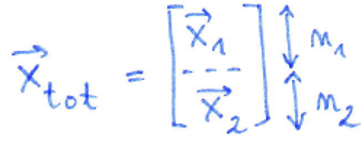
\includegraphics[width=0.4\textwidth]{Include/Figure/26.png}
\end{figure}

\textbf{On obtient ainsi typiquement des "matrices bloc" : }\\


$
\begin{cases}
	\dot{\vec{x_{tot}}} = A_{tot}\vec{x_{tot}} + B_{tot} u \\
	y = C_{tot}\vec{x_{tot}} + D_{tot}u
\end{cases}
$
\hfill
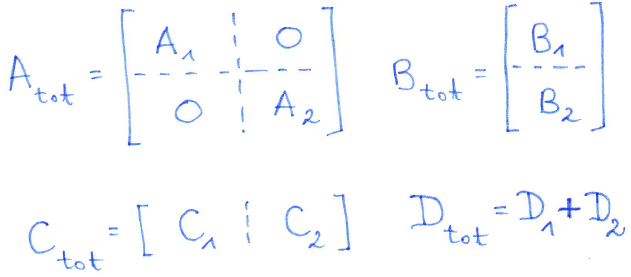
\includegraphics[width=0.6\textwidth]{Include/Figure/28.png}\\


\subsubsection{Exemple : mise en cascade}
\begin{figure}[H]
    \centering
    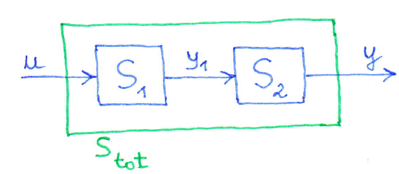
\includegraphics[width=0.5\textwidth]{Include/Figure/29.png} \hfill
    \hfill 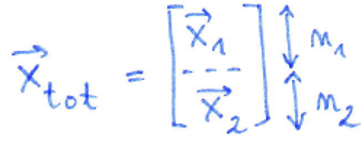
\includegraphics[width=0.4\textwidth]{Include/Figure/26.png}
\end{figure}

\begin{flushleft}
\textbf{Donné : } $A_1,\;B_1,\;C_1,\;D_1,\;A_2,\;B_2,\;C_2,\;D_2$\\
\textbf{Trouver :} $ A_{tot}, \;B_{tot}, \;C_{tot}, D_{tot}$ ? \\
\end{flushleft}


\subsection{Conversion "espace d'état" $\rightarrow$ "fonction de transfert"}

Rappel : 
\begin{equation}
\boxed{
\begin{array}{l r}
	\frac{1}{S} \; : \; Intgrateur & S \; : \; dérivateur 
\end{array}}
\end{equation}

\begin{equation}
	\begin{array}{l c l}
	\dot{x}(t) & = & Ax(t) + Bu(t)  \\
	\; & \downarrow  & \;\\
	\; & \mathscr{L} & \;\\
	\; & \downarrow  & \;\\
	S \cdot I \cdot X(S) & = & AX(S) + BU(S) \\
	(sI-A)X(S) & = & BU(S) \\
	X(S) & = & (SI-A)^{-1}BU(S)\\
	y(t) & = & Cx(t) + Du(t)\\
	Y(S)	 & = & CX(S) + DU(S)\\
	\end{array}
\end{equation}

\begin{equation}
	\Rightarrow G(S) = C(SI-A)^{-1}B + D
\end{equation}

\begin{equation}
	\lim_{s \rightarrow \infty} = D \; \hat{=} \; gain \; haute \; frequence
\end{equation}

\begin{equation}
	gain \; statique \; G(s=0)=-CA^{-1}B+D
\end{equation}

\subsubsection{Exemple double intégrateur}

\begin{figure}[H]
    \centering
    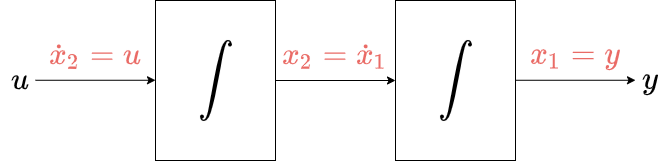
\includegraphics[width=0.5\textwidth]{Include/Figure/31.png}
\end{figure}
	
\begin{equation}
\begin{array}{l c c}
		\dot{x_1} = x_2 & \; & \dot{x} \; = \; Ax + Bu \\
		\dot{x_2} = u   & \Rightarrow & y       \; = \; Cx + Du\\
		x_1 = y
\end{array}
\end{equation}
	
\begin{equation}
\begin{array}{c c c c}
	A = \begin{bmatrix}
	0 & 1 \\ 0 & 0
	\end{bmatrix} & B = \begin{bmatrix}
	0 \\ 1
	\end{bmatrix} &
	C = \begin{bmatrix}
	1 & 0
	\end{bmatrix} &
	D = 0
\end{array}
\end{equation}


\begin{flushleft}
	Rappel : $G(S) = C(SI-A)^{-1}B + D$
\end{flushleft}

\begin{center}
$ (SI-A)^-{1} = (\begin{bmatrix} S & 0 \\ 0 & S \end{bmatrix} - \begin{bmatrix} 0 & 1 \\ 0 & 0 \end{bmatrix})^{-1} = \frac{1}{S^2} \begin{bmatrix} S & 1 \\ 0 & S \end{bmatrix} $
\end{center}

\begin{center}
$ C(SI-A)^{-1}B = \frac{1}{S^2} \begin{bmatrix} S & 1 \\ 0 & S \end{bmatrix} \cdot \begin{bmatrix} 0 \\ 1 \end{bmatrix} = \begin{bmatrix} \frac{1}{S^2} \\ \frac{1}{S^2} \end{bmatrix} $
\end{center}

\begin{center}
$ C(SI-A)^{-1}B + D = \begin{bmatrix} 1 & 0 \end{bmatrix} \cdot \begin{bmatrix} \frac{1}{S^2} \\ \frac{1}{S^2} \end{bmatrix} + 0 = \frac{1}{S^2} $
\end{center}

\begin{center}
	$ \boxed{G(S) = C(SI-A)^{-1}B + D = \frac{1}{S^2}} $
\end{center}
	

\subsection{Transformée en $\mathscr{Z}$}

\begin{equation}
	\begin{cases}
		x[k+1] = A_nx[k] +B_u[k] \\
		y[k] = C_nx[k] + D_nu[k] 
	\end{cases}
\end{equation}
\begin{center}
$\Downarrow \mathscr{Z}$
\end{center}

\begin{equation}
\begin{array}{c}
	z I X(z) = A_n X(z) + B_n U(z) \\[6pt]
	(z I - A_n)X_n(z) = b_n U(Z) \\[6pt]
	X_n(z) = (zI-A)^{-1} B_nU(z) \\	[6pt]
	Y(z) = (C(zI-A)^{-1}B_n + D_n)U(z)
\end{array}
\end{equation}

Le gain statique est donné par: \\
\begin{equation}
	\boxed{G(z = 1)=C_n(zI-A)^{-1}B_n + D_n}
\end{equation}

\begin{equation}
	\boxed{\text{Rappel : }z = e^{s \cdot h}}
\end{equation}

\subsection{Pôles = valeurs propres de A}
\begin{center}
	$\boxed{G(S) = C(SI-A)^{-1}B + D}$ \\
\end{center}

La matrice inverse de $(SI-A)$ fait intervenir le \textbf{polynôme caractéristique} \textbf{det$(SI-A)$} au dénominateur. Une valeur de $S$ qui annule le dénominateur est appelée \textbf{pôle} de la fonction ou matrice de transfert.\\

Les \textbf{pôles} correspondent aux \textbf{valeurs propres} de $A$, c'est à dire les racines du \textbf{polynôme caractéristique} \textbf{det$(SI-A) = 0$}.\\

Les \textbf{pôles} traduisent essentiellement le \textbf{comportement dynamique du système} :
\begin{itemize}
\item stable / instable
\item rapide / lent
\item oscillant / non oscillant
\end{itemize}

\subsection{Stabilité des systèmes}
Un système LTI est stable si sa réponse impulsionnelle revient à l'origine : \\
\begin{itemize}
	\item Temps continue : Si la partie réel de tous les \textbf{pôles} du système se trouvent dans le \textbf{demi-plan gauche} du plan complexe $\boxed{\text{Re}(P) < 0}$ 
	\item Temps discret : Si les tous les \textbf{pôles} du système se trouvent à \textbf{l'intérieur du cercle unitaire} $\boxed{\vert z \vert < 1}$
\end{itemize}
La relation en entre constante de temps et pôles pour temps continue:
\begin{equation}
	\tau = \frac{-1}{\text{Re}(P)}
\end{equation}
Avec $\text{Re}(P) \; =$ partie réelle d'un pôle du système $\rightarrow$ valeurs qui annule le dénominateur de la fonction de transfert.

\subsubsection{Exemple 1}
Pour une matrice \textbf{triangulaire} ou \textbf{diagonale}, les \textbf{pôles} correspondent aux \textbf{éléments sur la diagonale} :

\begin{figure}[H]
    \centering
    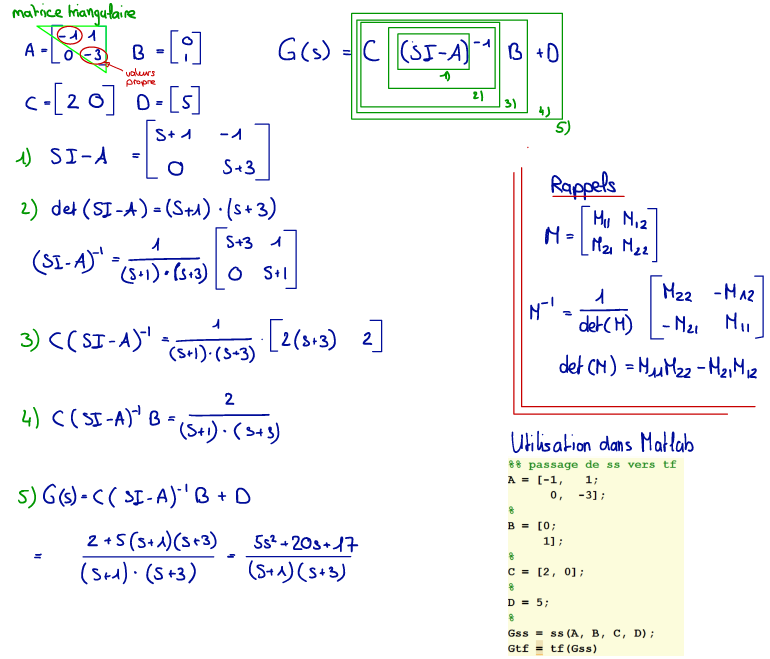
\includegraphics[width=0.9\textwidth]{Include/Figure/32.png}
\end{figure}

\subsubsection{Exemple 2}

\begin{figure}[H]
    \centering
    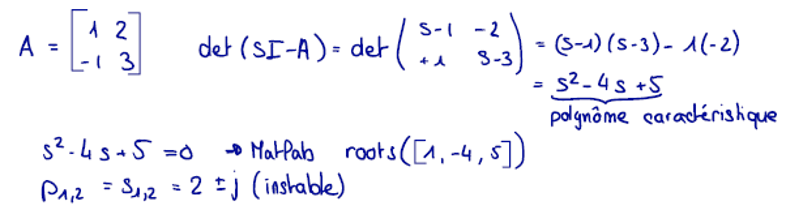
\includegraphics[width=\textwidth]{Include/Figure/33.png}
\end{figure}


\end{document}